\documentclass{book} % Definisi jenis dokumen

%%%%% Definisi paket-paket yang seharusnya digunakan %%%%%
\usepackage[utf8]{inputenc} % paket encoding input utf8
\usepackage[T1]{fontenc} % paket encoding huruf latin
\usepackage{tocbibind} % paket toc terdaftar dalam toc

%%%%% Definisi paket-paket yang digunakan sesuai kebutuhan %%%%%
\usepackage[yyyymmdd,hhmmss]{datetime} % paket tanggal-waktu
\usepackage{geometry} % paket ukuran kertas dan margin
\usepackage{graphicx} % paket grafik/gambar
\usepackage{subcaption} % paket untuk subfigure
\usepackage{minted} % paket untuk source code
\usepackage{xcolor} % paket buat warna
\usepackage{hyperref} % paket buat link-link an

%%%%% Pengaturan ukuran kertas dan margin %%%%%
\geometry{
	a4paper,
	left=10mm,
	right=10mm,
	top=15mm,
	bottom=15mm,
}

%%%%% Pengaturan perintah informasi perangkat lunak (hanya untuk GNU/Linux) %%%%%
\newcommand{\ShowOsVersion}{
	\immediate\write18{\unexpanded{foo=`uname -sro` && echo "${foo}" > tmp.tex}}
	\input{tmp}\immediate\write18{rm tmp.tex}
}

\newcommand{\ShowTexVersion}{
	\immediate\write18{\unexpanded{foo=`pdflatex -version | head -n1 | cut -d' ' -f1,2` && echo "${foo}" > tmp.tex}}
	\input{tmp}\immediate\write18{rm tmp.tex}
}

\definecolor{LightGray}{gray}{0.95}

\hypersetup{%
	pdfborder = {0 0 0}
}

\begin{document}
	%%%%%%%%%%%%%%%%%%%%%%%%%%%%%%%%%%%%%%%%%%%%%%%%%%%%%%%%%%%%%%%%%
	
	\frontmatter % untuk halaman cover
	
	\begin{titlepage}
		
		\centering % untuk membuat tengah teks
		
		{
			\LARGE % pakai font besar
			\bf % pakai font BOLD
			Rangkuman Kegiatan Pengembangan Telemetri Vibrasi
		}
		
		\bigskip
		{\Large \bf Achmadi ST MT}
		\vfill % menambahkan ruang kosong vertikal
		
		\includegraphics[width=300pt]{images/vibslogo}
		\vfill
		
		\raggedright
		\noindent Dokumen ini ditulis dengan:\\ % tanda \\ menambahkan garis baru
		OS : \ShowOsVersion \\
		TeX : \ShowTexVersion \\
		Update: {\today} at \currenttime\\
	\end{titlepage}
	
	%%%%%%%%%%%%%%%%%%%%%%%%%%%%%%%%%%%%%%%%%%%%%%%%%%%%%%%%%%%%%%%%%
	
	\newpage % halaman baru
	\tableofcontents % daftar isi
	\listoffigures % daftar gambar
	\listoftables % daftar table
	
	%%%%%%%%%%%%%%%%%%%%%%%%%%%%%%%%%%%%%%%%%%%%%%%%%%%%%%%%%%%%%%%%%
	
	\mainmatter % pindah format halaman dari romawi ke angka (konten utama)
	
	\newpage
	\chapter{Goal}
	
	\section{Diagram Sistem}
	
	Berikut rangkuman tujuan akhir pengembangan:
	
	\begin{figure}[!ht]
		\centering
		\includegraphics[width=0.8\textwidth]{images/goal_diagram/goal}
		\caption{Diagram Pembangunan Sistem Monitoring}
	\end{figure}
	
	\section{Pemilihan Komponen}
	
	\subsection{Sensor Vibrasi}
	
	Sensor Vibrasi menggunakan TE-850M1:
	
	\begin{itemize}
		\item Analog Output 
		\item VDD Level Voltage (3.3V)
		\item Triaxial on separate
		\item Up to 25G vibration
	\end{itemize}
	
	\newpage
	\subsection{Microcontroller}
	
	Microcontroller menggunakan seri STM32Fx LQFP64:
	
	\begin{itemize}
		\item Arsitektur ARM Cortex-M
		\item VDD Level Voltage (3.3V)
		\item PLL hingga 72MHz
		\item ADC hingga 12bit
		\item Memiliki mode sleep dengan konsumsi rendah
		\item Harga terjangkau
	\end{itemize}
	
	\subsection{Transceiver}
	
	Module Radio Transceiver menggunakan seri LoRA SX1278:
	
	\begin{itemize}
		\item VDD Level Voltage (3.3V)
		\item Konsumsi daya rendah
		\item Frekuensi 433MHz (Kategori Pita 31 menurut UU Kominfo Tahun 2018)
		\item Termasuk non-3GPP sehingga tidak overlap dengan jaringan selular.
		\item Dapat menjangkau area hingga radius 10km (RSSI minimal)
		\item Harga terjangkau
	\end{itemize}
	
	\newpage
	\chapter{Development Stages}
	
	\section{Sensor Testing}
	
	Tahapan ini bertujuan untuk menguji antar muka sensor vibrasi TE-850M1 ke STM32.
	
	\subsection{Setup Pengujian}
	
	\begin{figure}[h]
		\centering
		\begin{subfigure}{0.3\textwidth}
			\includegraphics[width=\textwidth]{images/vibparts.png}
			\caption{Mockup}
		\end{subfigure}
		\begin{subfigure}{0.3\textwidth}
			\includegraphics[width=\textwidth]{images/vibs.png}
			\caption{Actual}
		\end{subfigure}
		\caption{Preview Unit}
	\end{figure}
	
	\begin{figure}[!ht]
		\centering
		\includegraphics[width=0.6\textwidth]{images/testing}
		\caption{Diagram Pengujian}
	\end{figure}
	
	\newpage
	\begin{figure}[h]
		\centering
		\includegraphics[width=0.65\textwidth]{images/testactual.jpg}
		\caption{Dokumentasi Testing}
	\end{figure}
	
	\subsection{Desain Purwarupa}
	
	
	
\end{document}